\documentclass{article}

\usepackage{tabularx}
\usepackage{booktabs}
\usepackage{graphicx}
\usepackage{paralist}
\usepackage{listings}
\usepackage{booktabs}
\usepackage{hyperref}
\usepackage{amsfonts}
\usepackage{amsmath}
\usepackage{color}
\usepackage{fancyhdr}
\usepackage{geometry}
\usepackage{soul}
\usepackage{multirow}
\usepackage{ulem}
\usepackage{float}

\title{SRS\\Digital Twin Forest}
\author{Yichen Jiang, Bowen Zhang, Jiacheng Wu, Junhong Chen, Tingyu Shi\\Team 8}

\begin{document}

\maketitle
%%%%%%%%%%%%%%%%%%%%%%%% Revision History %%%%%%%%%%%%%%%%%%%%%%%%%%%%%%%
\newpage
\begin{table}[htp]
\caption{Revision History} 
\begin{tabularx}{\textwidth}{llX}
\toprule
\textbf{Date} & \textbf{Developer(s)} & \textbf{Change}\\
\midrule
Sept 24, 2022 & All team members & Initial Document\\
Sept 26, 2022 & All team members & Update Requirements\\
Sept 29, 2022 & All team members & Revision 0\\

\bottomrule
\end{tabularx}
\end{table}
%%%%%%%%%%%%%%%%%%%%%%%%%%%%%%%%%%%%%%%%%%%%%%%%%%%%%%%%%

\vspace{8cm}

%%%%%%%%%%%% Template Name %%%%%%%%%%%%%%%%%%%%%%%%%%%%%%%
\noindent This document follows \href{https://www.cs.uic.edu/~i440/VolereMaterials/templateArchive16/c\%20Volere\%20template16.pdf}{\textcolor{red}{Volere Template}}.
The following are some modifications that we made to the 
original template:\\
Our team skipped "Business Data Model and Data Dictionary" because our team will
go to the actual forest to measure the data in mid October. Also, our team will
discuss with Dr. Gonsamo about what data need to be added to the virtual forest
representation as the project progresses. Currently, our team focuses on modelling.
We will add this part in Revision 1.
%%%%%%%%%%%%% Template Name End %%%%%%%%%%%%%%%%%%%%%%%%%%%%


\newpage
%%%%%%%%%%%%%%Contents%%%%%%%%%%%%%%%%
\tableofcontents
\listoftables
\listoffigures
\cleardoublepage

%%%%%%%%%%% Project Drivers %%%%%%%%%%%%
\section{Project Drivers}
\subsection{The purpose of the Project}
\subsubsection{The User Business or Background of the Project Effect}
A digital twin is a virtual representation of the real world, including physical objects, 
processes, relationships, and behaviors. Elements of a digital twin include data capture
and integration, visualization, advanced analysis including AI, automation, and information
sharing and collaboration. This project can be beneficial for two groups of users.  The first
group of users is forest owners. This project can help them to manage the forest. The 
second group of users is meteorologists. This project can help them to 
do research.
\subsubsection{Goals of the Project}
\begin{itemize}
    \item Implement the virtual forest, which corresponds to the target natural forest. The model of a single tree is obtained by LiDAR scanning on the field. The final project combines previous models and lab statistics to give a virtual view of the forest. 
    \item Provide basic representation of data, such as age, height, plant density, 
    etc. 
\end{itemize}

\subsection{Stakeholders}
\subsubsection{The client}
\begin{itemize}
    \item Dr. Alemu Gonsamo from School of Earth, Environment and Society McMaster University. (Dr. Gonsamo is the supervisor of this project.)
    \item Dr. Spencer Smith from Computing and Software Department, McMaster University. (Dr. 
    Smith is the professor of capstone course, and he will give assessments of this project.)
\end{itemize}
\subsubsection{The Customer}
\begin{itemize}
    \item Forest Owners(The final project can be helpful for forest owners to better manage the 
    forest and make decisions)
    \item Meteorologists(The final product can be helpful for researchers to 
    study climate change)
\end{itemize}
\subsubsection{Other Stakeholders}
\begin{itemize}
    \item Dr. Gonsamo's lab members(Graduate students from the lab will provide suggestions and
    data needed to assist this project)
\end{itemize}
\subsubsection{The Hands-On Users of the Product}
The hands-on users of this product are the same as customers mentioned in section 1.2.2. Users'
responsibilities are also mentioned in section 1.2.2. For subject matter experience, these 
users are master. For both forest owners and meteorologist, they are definitely
familiar with the real forest and our product can help them better doing
their jobs. For the point of technology, we assume that they 
have little experience of virtual representation
technologies.
\subsubsection{Personas}

\begin{itemize}
    \item Dr. Aly is an 55-year-old assistant professor working in a university, living with his family near his lab. His research mainly focuses on remote sensing of vegetation, global change ecology, and climate change impact. His research is supported by an association of several forest owners, who are willing to let Dr. Aly locate part of researches and collect needed information in their forest. If he needs to go to the field that day, the typical schedule of him is to get up on 6am, take 90 minutes to commute to the target forest with some students he supervises, collect and record data there, and come back to his lab with another 90 minutes. 
    
    Dr. Aly's goals are to find a convenient way to free him from frequent commuting, and to look for a new method to manage and visualize all the significant data for a purpose of teaching. 
    
    \item Mrs. Miller owns 40-acre land including a 2-acre forest. She is now 36 years old and lives with her husband, who works as a financial analyser, in Toronto. She runs a coffee house as a full-time job, and drives to her forest every two months to check everything's fine. Though she cares about her forest, spending over three days every two months to go through every area seems impossible for her, she would love to have a new method to manage her forest and get updated information regularly, in order to make better strategies for the forest. 
\end{itemize}


\subsubsection{Priorities Assigned to Users}
\begin{itemize}
    \item Key Users: Dr. Gonsamo, Forest owners, meteorologist
    \item Secondary Users: Dr. Smith, Lab members
\end{itemize}
\subsubsection{User Participation}
\begin{itemize}
    \item Dr. Smith: Dr. Smith will provide suggestions about project management, project 
    documents and project technologies like git.
    \item Dr. Gonsamo: Dr. Gonsamo will provide business knowledge(forest data), 
    interface prototyping and usability requirements for this project. Since Dr. Gonsamo is 
    a meteorologist, he can also provide suggestions for meteorologists.
    \item Lab members: Lab members will help this project by providing some business knowledge
    about the forest.
    \item Forest Owners: Forest owners can provide commercial data about the forest. Commercial
    data include tree cutting data, annual profits, etc.
\end{itemize}
\subsubsection{Maintenance Users and Service Technicians}
The project members will be responsible for maintaining and changing the product.
%%%%%%%%%%% Project Drivers End %%%%%%%%%%


%%%%%%%%%% Project Constraints %%%%%%%%%%%%
\section{Project Constraints}
\subsection{Mandated Constraints}
\subsubsection{Solution Constraints}
\begin{itemize}
    \item Scanning Technology: Our team will use Light Detection and Ranging(LiDAR) method
    to scan physical objects in the forest. This is a kind of Laser Scanning technology. 
    We determined to use this technology for three reasons. First, LiDAR sensors
    are accessible because they are common among Apple devices like iPhone or iPad. The 
    second reason is that LiDAR sensors can provide accurate scanning. The third reason
    is that LiDAR allows to scan large areas within a short period of time.
    \item Modeling Technology: Our team will use Unity for modeling task. Unity version 
    will be 2021.3. Our team members use different platforms(Windows or MacOS). Unity is 
    suitable for our team because it is a cross-platform software. Also, Unity has existing packages which can speed up our modelling process.
    \item Project Documents Technology: Our team will use \LaTeX for our documents.
    \item Project Cooperation Technology: Our team will use GitHub to cooperate.
    \item Code Testing Technology: VS2019 will be used for the unit test. The team will create a unit test project (.NET Framework) that contains MSTest unit tests.
    \item Code Coverage Testing Technology: The JetBrains dotCover is a code coverage tool that integrates with VS2019. It can execute and run coverage analysis for unit tests in Visual Studio.
\end{itemize}
\subsubsection{Implementation Environment of the Current System}
The product will be installed in different operating systems such
as Windows, MacOS, iPadOS, iOS and Android.
\subsubsection{Partner or Collaborative Applications}
N/A(Our product is an independent product)
\subsubsection{Off-the-Shelf Software}
\begin{itemize}
    \item LiDAR: iPad Pro LiDAR should be used to scan the forest and collect data
    for modelling.
    \item Unity: Unity should be used for modelling and post processing.
    \item Agisoft metashape: It should be used for modelling.
\end{itemize}
\subsubsection{Anticipated Workplace Environment}
Both indoor and outdoor are possible workplace environments. In order to 
improve the convenience for outdoor workplace environments, 
the product should be compatible with mobile devices such
as cell phones or tablets.
\subsubsection{Schedule Constraints}
Please check our project schedule \href{https://github.com/wuj187/DigitalTwinCAS/tree/main/docs/DevelopmentPlan/Project_Schedule}{\textcolor{red}{here}}. The following are deadlines for demonstrations:
\begin{itemize}
    \item Proof of Concept Demonstration: 2022, Nov, 14
    \item Final Demonstration: 2023, Mar, 20
\end{itemize}
\subsubsection{Budget Constraints}
Total expenses should not exceed \$750.
\subsubsection{Enterprise Constraints}
N/A This project is not invested by any enterprise.
\subsection{Naming Conventions and Definitions}
\begin{itemize}
    \item LiDAR: Light Detection and Ranging(Scanning Technology)
    \item Plot: A square shaped area in the forest. There are 13 plots in total. 
    \item Target Forest: The natural forest modelled in this product.
    \item Digital Twin Forest: The virtual representation of the target forest.
    \item Update local data: The users are allowed to update any data on their own device. The update made by a user will not be updated to the other users.
    \item Update official data: The developing team would release updates regularly. The update made by the developing team can be updated to all users if they accept the latest version.
    \item Overall forest data: These are data for the whole forest. For example,
    these data may include overall $CO_2$ concentration or plant density of the whole
    forest.
    \item Forest plot data: The target forest is separated into 13 plots. Plot forest
    data
    has the same data types as the overall forest data, however, all the data are for
    a specific forest plot.
    \item Tree parameters: Tree parameters include data such as tree ages,
    perimeters,
    heights, species, etc.
\end{itemize}

\subsection{Relevant Facts and Assumptions}
\subsubsection{Relevant Facts}
\begin{itemize}
    \item Forest data keep changing all the time, but our 
    system will only update weekly. Therefore, the 
    system may not be able to reflect the most accurate data. 
    However, since the forest data will not change dramatically
    within a short period of time, the system should be 
    close to the real forest.
    \item The product can be beneficial for meteorologists to do research.
    \item The product can be beneficial for forest owners 
    to better manage the forest.
\end{itemize}
\subsubsection{Business Rules}
N/A
\subsubsection{Assumptions}
\begin{itemize}
    \item The scanning devices are available.
    \item Drones can be used for large area scanning.
    \item Unity and required toolboxes 
    should be accessible to all developers'
    devices.
    \item Users will use our product on Windows, MacOS, iOS, iPadOS,
    or Android.
    \item Forest data will not change dramatically within a 
    short period of time. 
    \item Virtual forest should be updated weekly for the 
    first year.
\end{itemize}
%%%%%%%%%%%% Project Constraints End %%%%%%%%%


%%%%%%%%%%% Functional Requirements %%%%%%%%%%%%
\section{Functional Requirements}
\subsection{The Scope of the Work}
\subsubsection{The Current Situation}
Currently, digital twin technologies are being utilized in many
areas, such as Aerospace and Aeronautics, manufacturing, automotive, etc. For more detailed information, please check paper \href{https://github.com/wuj187/DigitalTwinCAS/blob/main/refs/DT_Applications.pdf}{\textcolor{red}{\textit{Applications of Digital Twin across 
Industries: A Review}}} in our reference folder. This paper talks about 
many applications of digital twin technologies in different areas.\\
After searching online, we found a similar product from Tietoery
Company called \href{https://www.tietoevry.com/en/industries/forest-pulp-paper-and-fibre/forest-solutions/wood-and-fibre-ecosystem-and-integration/digital-forest-twin/}{\textcolor{red}{Digital Forest Twin}}.
According to its introduction, this product can 
be accessed using head mounted devices or
web browsers, which is different from our product. Also, 
from the company's website, we can know little details about how
 this product works. Therefore, our team does not know too much
 about existing business processes.
 \newpage
\subsubsection{The Context of the Work}
The following is the context of use diagram:
\begin{figure}[H]
\begin{center}
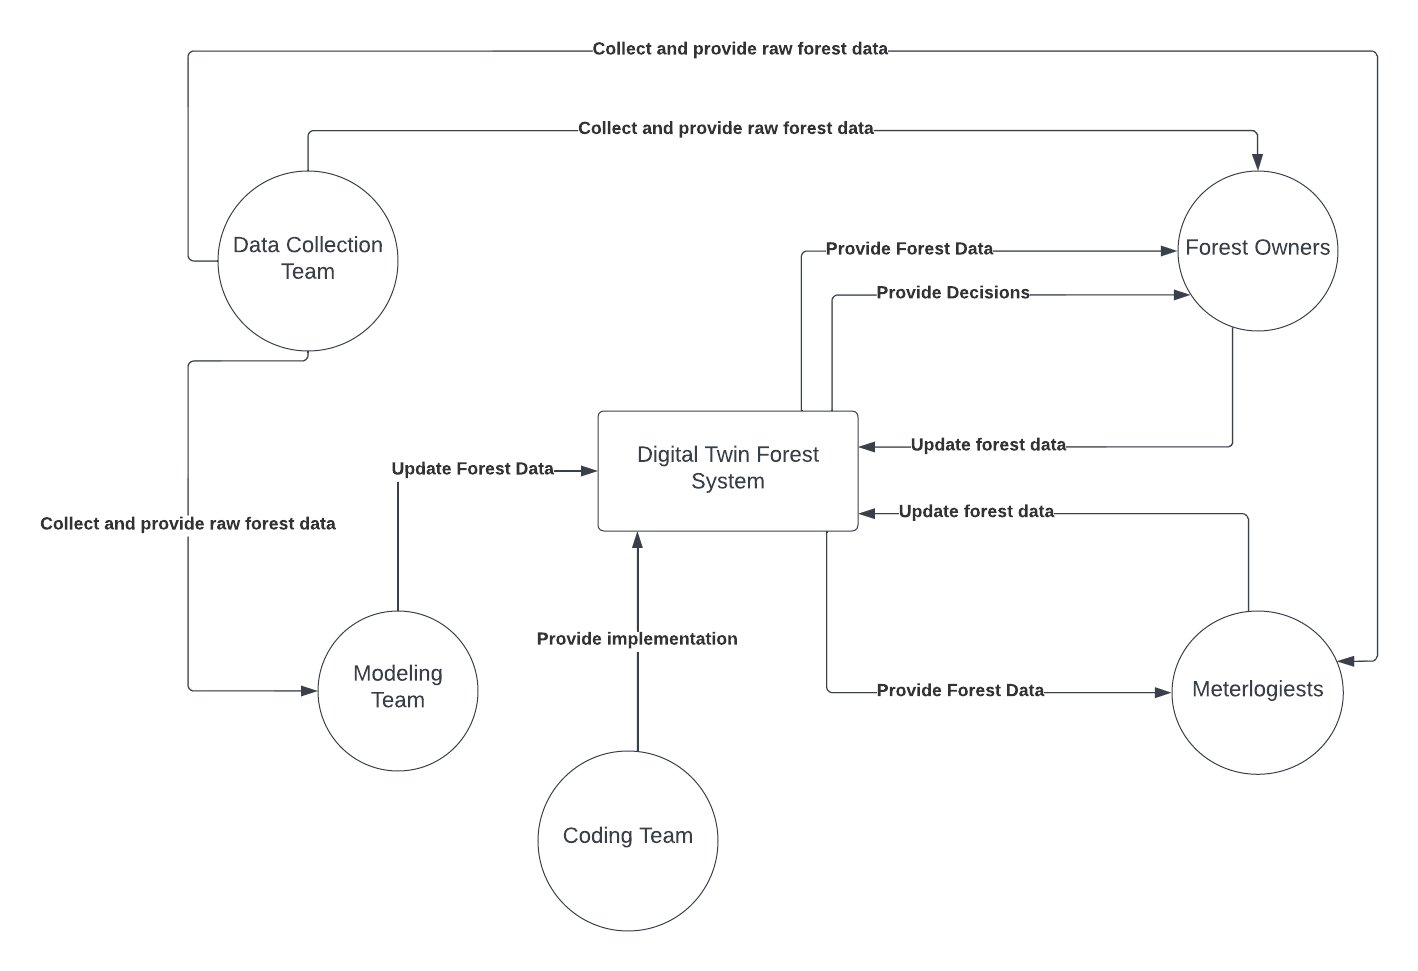
\includegraphics[scale=0.7]{SRS_Pictures/Context_Use.png}
\end{center}
\caption{Context Diagram}
\end{figure}

\noindent If the above picture is not clear, please download the picture \href{https://github.com/wuj187/DigitalTwinCAS/blob/main/docs/SRS/SRS_Pictures/Context_Use.png}{\textcolor{red}{here}}. \\

\noindent Forest data includes the following:
\begin{itemize}
    \item Forest atmosphere data (eg. $CO_2$ concentration)
    \item Forest measurements (eg. distance between different trees)
    \item Tree parameters(eg. height, trunk perimeter, age, speices)
    \item Forest soil data
    \item Plant density
\end{itemize}
As the project progresses, we may add more data to our virtual forest representation.

\subsubsection{Work Partitioning}
\begin{table}[H]
\caption{Business Event List} 
\begin{tabularx}{\textwidth}{XXX}
\toprule
\textbf{Event Name} & \textbf{Input and Output} & \textbf{Summary of BUC}\\
\midrule
Forest scanning & Forest data(in) & Scan the forest and generate data for modelling.\\
Import models & Forest models(in) & Edit and upload new models to the system.\\
Code implementation & System modules(in) & Add new modules to the system.\\
Update data & Forest Data(in) & Replace the old data in the system with new data.\\
Data visualization & Forest Data(output) & The system demonstrates the organized data to the users.\\
Decision Making & Forecast and suggestions (output) & The system generates reports based on the given data.\\
\bottomrule
\end{tabularx}
\end{table}

\newpage
\subsubsection{Specifying a Business Use Case (BUC)}
The following is an activity diagram to indicate how users can check various data
from the system\\
\begin{figure}[H]
    \centering
    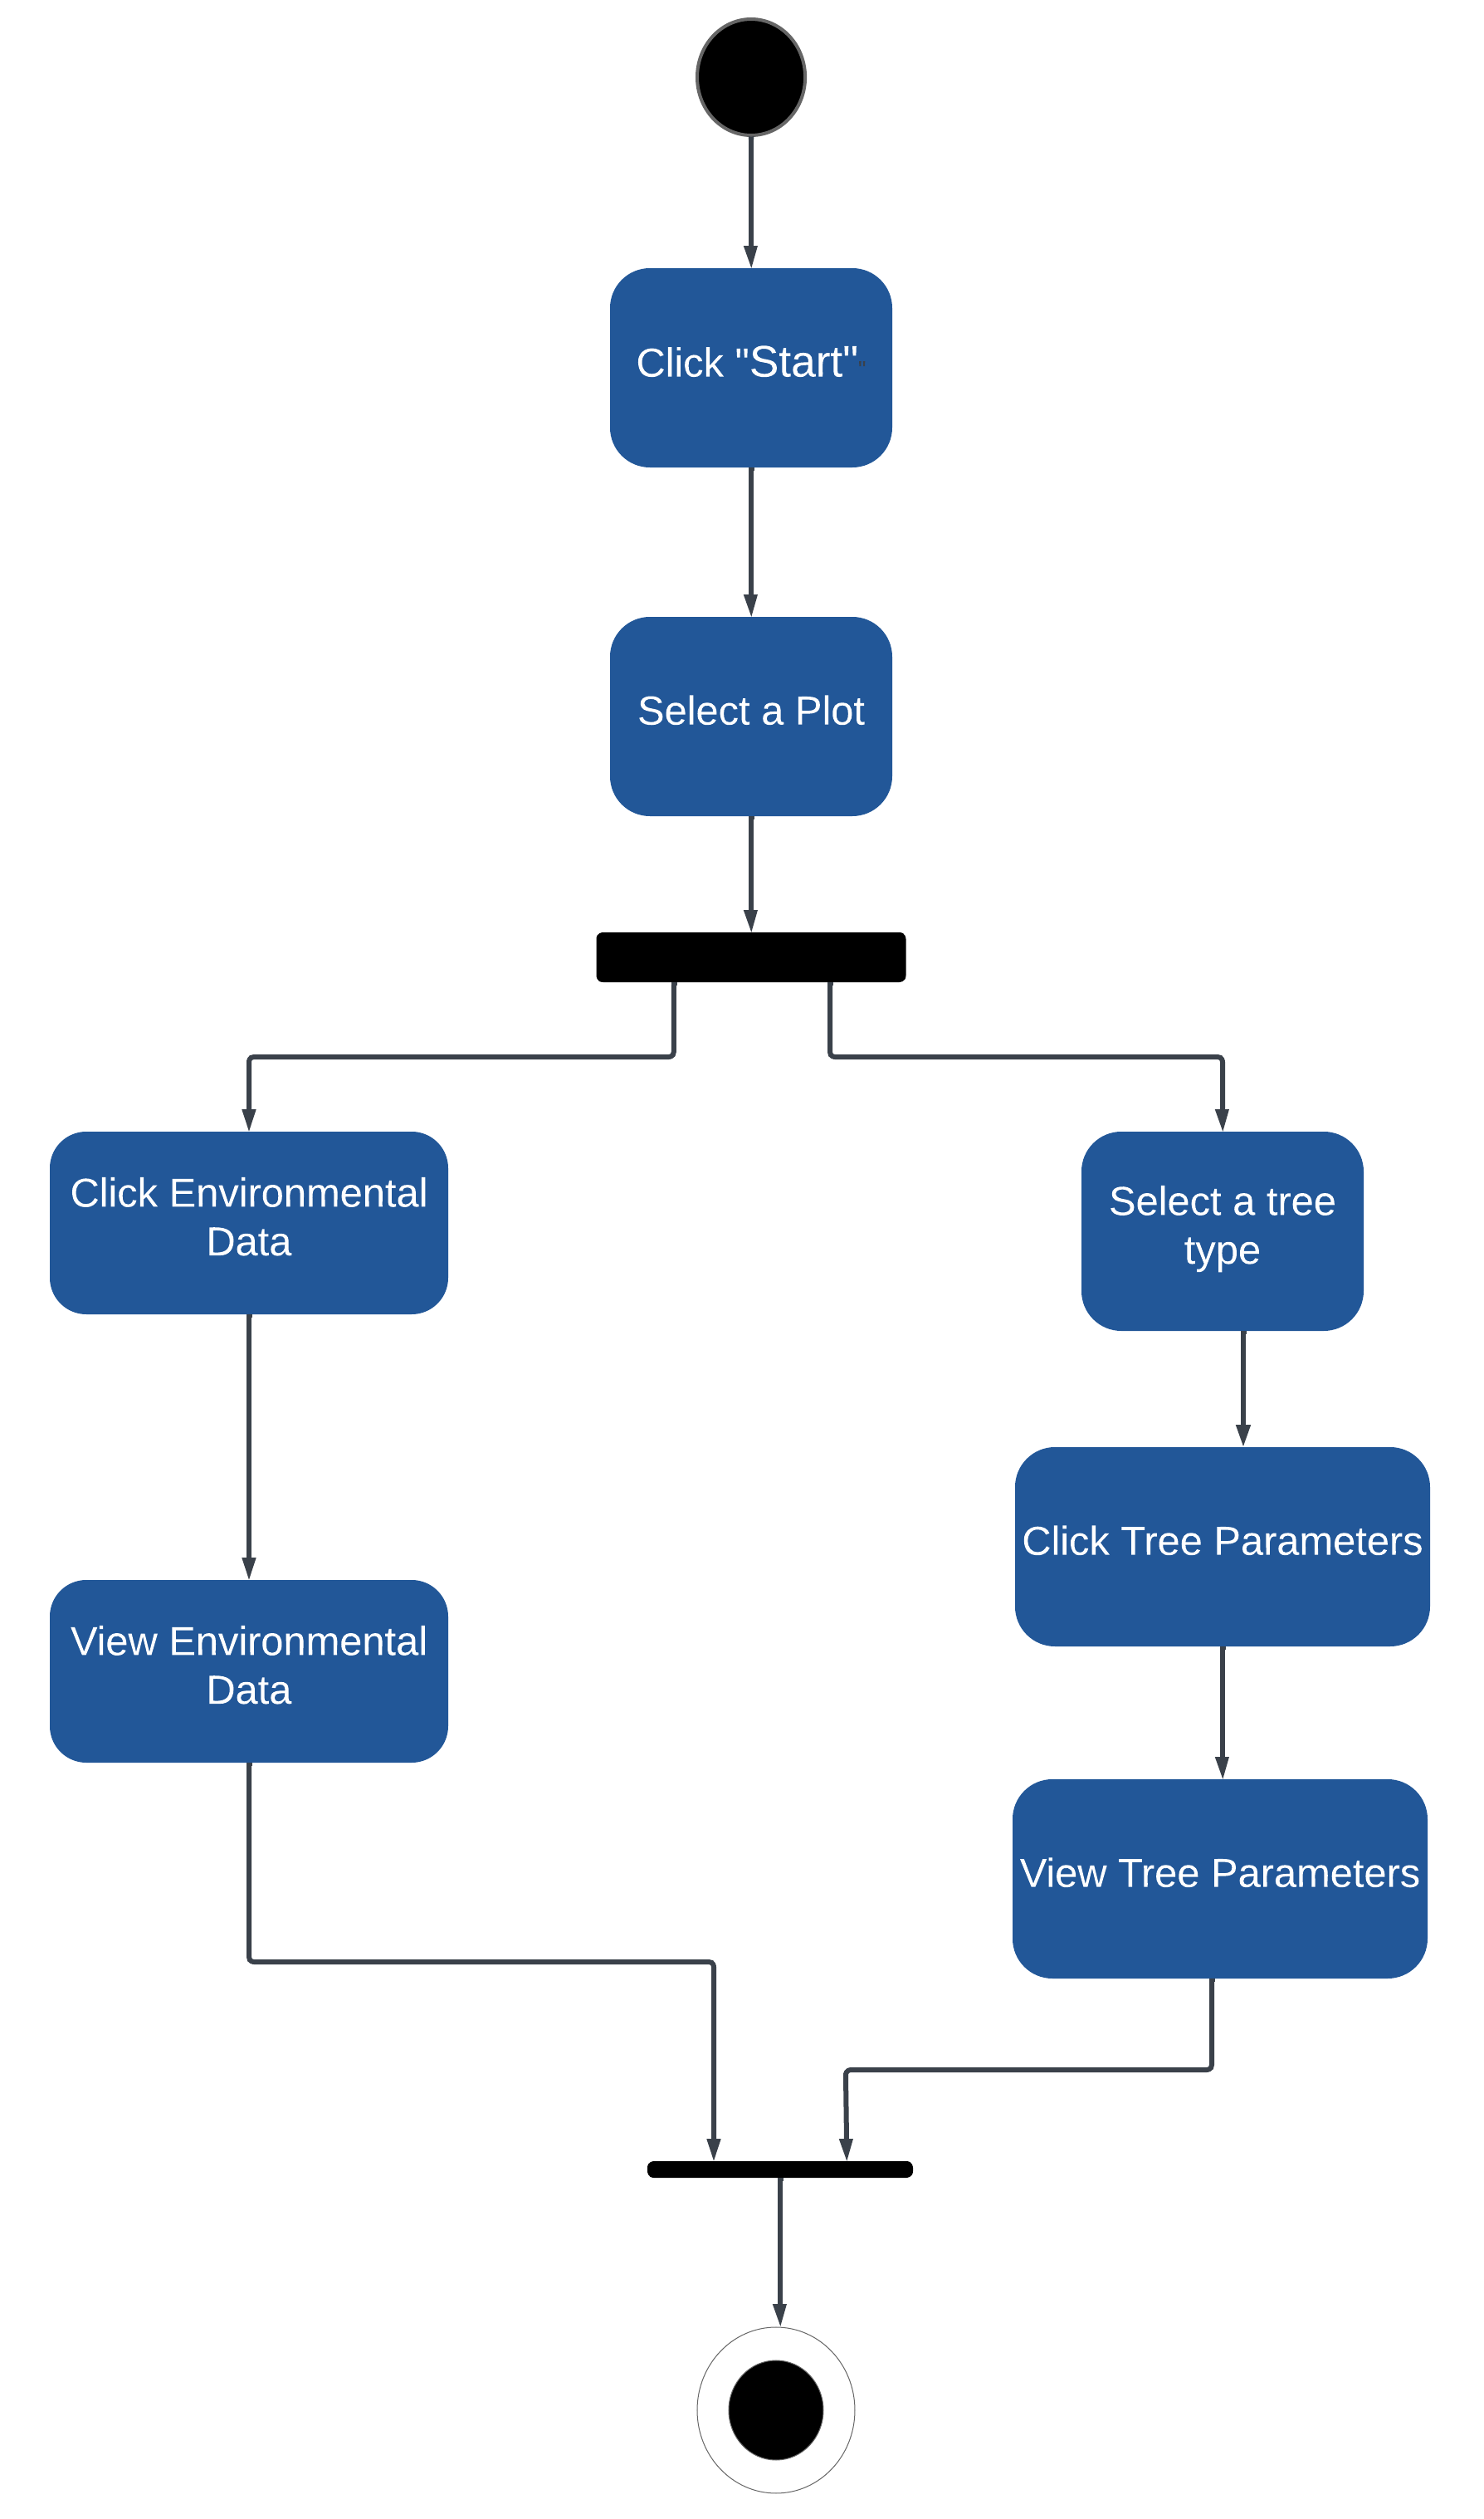
\includegraphics[scale=0.8]{SRS_Pictures/Activity_Diagram.png}
    \caption{An activity diagram to show how users can check data}
\end{figure}
\noindent If the above picture is not clear, please download the picture \href{https://github.com/wuj187/DigitalTwinCAS/blob/main/docs/SRS/SRS_Pictures/Activity_Diagram.png}{\textcolor{red}{here}}.

\subsection{The Scope of the Product}
\subsubsection{Product Boundary}
\begin{figure}[H]
    \centering
    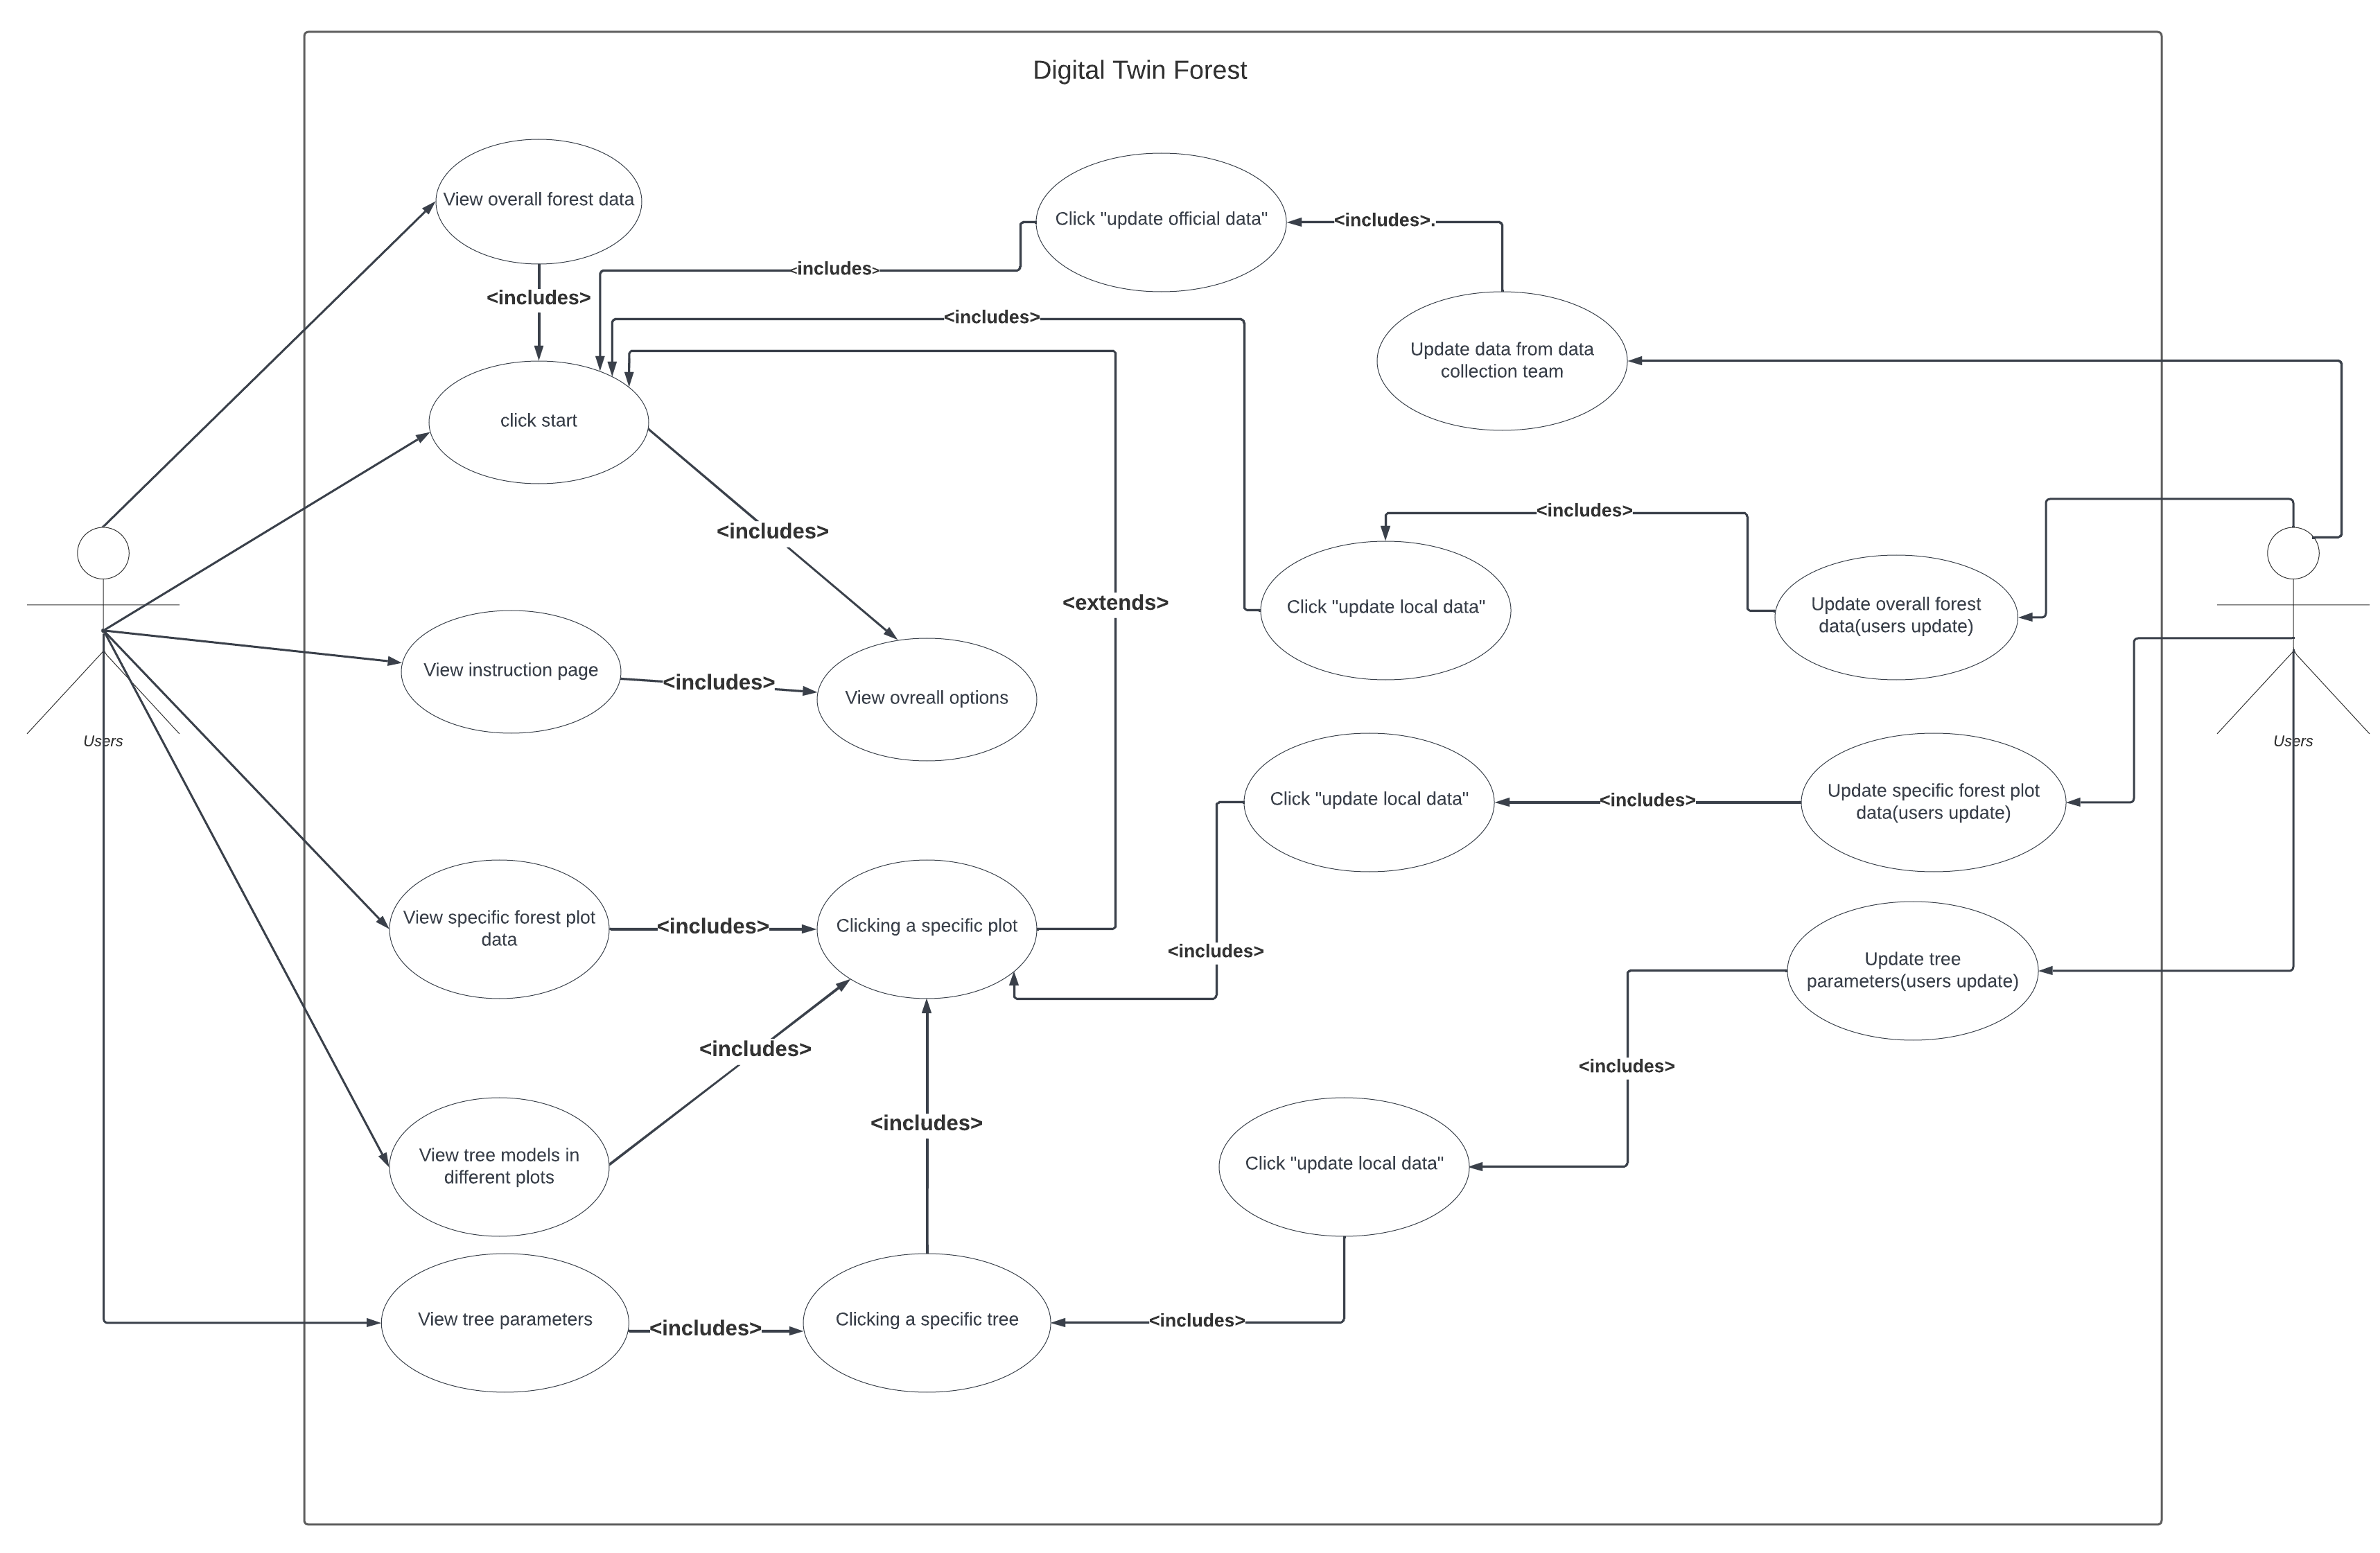
\includegraphics[scale=0.3]{SRS_Pictures/Use_Case.png}
    \caption{Use Case Diagram}
\end{figure}
\noindent If the above picture is not clear, please download the picture \href{https://github.com/wuj187/DigitalTwinCAS/blob/main/docs/SRS/SRS_Pictures/Use_Case.png}{\textcolor{red}{here}}.

\subsubsection{Product Use Case Table}
\begin{enumerate}
    \item PUC Name: View overall forest data\\
    Actor: Users\\
    Input: Users click "start" at the beginning of the application.\\
    Output: Overall forest data appear in the windows at two sides of the screen. 
    \item PUC Name: Click start\\
    Actor: Users\\
    Input: Users click "start" at the beginning the application.\\
    Output: 13 plots and overall forest data appear on the screen.
    \item PUC Name: View instruction page\\
    Actor: Users.\\
    Input: Users click "Instruction" at the beginning the application.\\
    Output: Instruction page appears on the screen. 
    \item PUC Name: View specific forest plot data\\
    Actor: Users.\\
    Input: Users click a specific forest plot.\\
    Output: Forest data of a specific plot appear in the windows at two sides of
    the screen. 
    \item PUC Name: View tree models in different plots\\
    Actor: Users.\\
    Input: Users click a specific forest plot.\\
    Output: Tree models of a specific plot appear on the screen.
    \item PUC Name: View tree parameters\\
    Actor: Users.\\
    Input: Users click a specific tree.\\
    Output: Tree parameters appear in a window beside the tree.
    \item PUC Name: Update data from data collection team\\
    Actor: Users.\\
    Input: Users click "update official data".\\
    Output: All the data(including overall forest data, forest plot data and tree 
    parameters) will be synchronized with the official data collected from the 
    data collection team.
    \item PUC Name: Update overall forest data(Users update)\\
    Actor: Users.\\
    Input: Users click "update local data" after clicking "start".\\
    Output: A window appears on the screen to let users update overall
    forest data.
    \item PUC Name: Update forest plot data\\
    Actor: Users.\\
    Input: Click "update local data" in a specific forest plot.\\
    Output:  A window appears on the screen to let users update
    forest plot data.
    \item PUC Name: tree parameters\\
    Actor: Users.\\
    Input: Click "update local data" in tree information windows.\\
    Output:  A window appears on the screen to let users update tree 
    parameters.
\end{enumerate}



\subsection{Functional Requirements}

\begin{enumerate}[FR1]
	\item The product must display the basic instruction when the user accesses to the product for the first time.\\
	\textbf{Rationale}: The user might not be familiar with our product especially when the user uses it for the first time.\\
	\textbf{Fit Criterion}: A basic instruction 
	option shows up on the user interface after the software is launched. 
	
	\item The product must allow the user to click a ‘start’ button to start the virtual tour.\\
	\textbf{Rationale}: The user would need a clear signal to get started.\\
	\textbf{Fit Criterion}: A 'start' button is displayed on the home page of the application.
	
	\item The product must load the forest model when the user clicks ‘start’.\\
	\textbf{Rationale}: The clicking of 'start' indicates the user has been through the instruction and ready to use our product. The product can now initialize the functions by loading the model.\\
	\textbf{Fit Criterion}: Once the user select 'start', the data of the forest is loaded.
	
	\item The product shall display a progress bar while loading. \\
	\textbf{Rationale}: The product should give feedback to the action of clicking 'start'. The loading might take seconds and a progress bar helps when the user's waiting. \\
	\textbf{Fit Criterion}: A dynamic progress bar will be displayed when the forest is loading.
	
	\item The product must display a full view of the digital twin forest.\\
	\textbf{Rationale}: Users might not be aware of the overall information and the overview of the forest that the product simulates.\\
	\textbf{Fit Criterion}: 13 complete plots of the forest with highlighted borders will show up together when the user zooms out the interface.
    
    \item The product must allow the user to minimize the user interface. \\
    \textbf{Rationale}: The user might want to pay more attention to the model instead of information related to it. Minimizing the user interface allows the user to do so. \\
	\textbf{Fit Criterion}: The windows of the user interface will be minimized to the side of the screen once the user clicks the \textit{minimized} button on the user interface.
	
	\item The product must display a menu to show specific data when the user clicks on each plot.\\
	\textbf{Rationale}: After the user has located a specific plot, he or she should be able to access to related information. And the most intuitive and convenient method to do so would be clicking. \\
	\textbf{Fit Criterion}: After the user clicks at a specific plot, windows containing information about that plot shall be displayed on both sides of the screen.
	
	\item The product must allow the users to click a specific tree in order to view related information.\\
	\textbf{Rationale}: It allows users to see the related information of a specific tree in detail.\\
	\textbf{Fit Criterion}: After the user enters a specific plot and clicks on a specific tree. windows containing information about that kind of tree shall be displayed on both sides of the screen. 
	
	\item The product must display the overall data of the forest on both sides of the screen.\\
	\textbf{Rationale}: The product should display the important data that our users might care about on the user interface, while should not let the information interrupt the display of model. So, it should distribute the information on both sides.\\
	\textbf{Fit Criterion}: When the full view of the forest is displayed, windows containing the overall information of the forest shall be shown on both sides of the screen. 
	
	\item The product must allow the users to zoom in and out of the model.\\
	\textbf{Rationale}: The user might need to zoom in to locate a specific plot or zoom out for a fuller view of the forest. \\
	\textbf{Fit Criterion}: When the user scrolls forward the scroll wheel of the mouse, the map shall be zoomed in. When the user scrolls backward, the map shall be zoomed out. 
	
	\item The product must allow the user to change the point of view. \\
	\textbf{Rationale}: The users might need to observe the forest from different perspectives.\\
	\textbf{Fit Criterion}: The user's point of view shall change when the user moves the mouse and scrolls the scroll wheel.
	
	\item The product shall display the information in separate pages when the content does not fit in one page.\\
	\textbf{Rationale}: The amount of information might not fit in a single page. Instead of compromising the user interface and minimizing the front size, displaying the information in several pages would be a better choice.\\
	\textbf{Fit Criterion}: Several pages will show up when showing information with very long content.
	
	\item The product shall allow the user to turn pages if the interface has multiple pages. \\
	\textbf{Rationale}: The user should be able to turn pages to switch among different sections of information.\\
	\textbf{Fit Criterion}: When showing multiple pages, page turn buttons shall be on each page. When the user clicks on the forward page turn button, the page shall display the previous information. When the user clicks on the backward page turn button, the page shall display the subsequent information.
	
	\item The product must allow the user to go back to the full view when focusing on a certain plot.
	\textbf{Rationale}: Users might need to go back to see the overview of the forest and see some overall information about the forest.  \\
	\textbf{Fit Criterion} The full view of the forest shall show up when the user scrolls backward the scroll wheel of the mouse.
	
	\item The product must allow the user to click an ‘exit’ button and quit the product.\\
	\textbf{Rationale}: The user would need a clear signal to exit.\\
	\textbf{Fit Criterion}: Once the user clicks on the 'exit' button, the application shall quit and the process of the software shall be terminated.
    
    \item The product must allow the user to update the information about the forest and trees.\\
	\textbf{Rationale}: In order to let the application show the latest information, it's necessary for users to upload the renew the information and statistics about the forest by themselves.\\
	\textbf{Fit Criterion}: After the user uploads the latest information, the virtual forest shall display this latest information. 
	
	\item The product must allow the user to choose to update the product or not when new version released.\\
	\textbf{Rationale}: Our product relies deeply on the latest information to give reasonable reference. The user can choose to update to the latest version when any version released.\\
	\textbf{Fit Criterion}: The product should overwrite any modification made by users and update all the information corresponding to the latest released version of our product.
	
\end{enumerate}
%%%%%%%%%%%%% Functional Requirements End %%%%%%%%%%%



%%%%%%%%%%%%% Non-functional Requirements %%%%%%%%%%%%%
\section{Nonfunctional Requirements}
\subsection{Look and Feel Requirements}
\subsubsection{Appearance Requirements}
\begin{enumerate}
    \item[LF1.1] The product shall have a goal that all modules adheres to.\\
    \textbf{Rationale}: The system can be consistent and coherent if all modules focus on one goal, and it's easy for users to understand the function of the system.\\
    \textbf{Fit criterion}:  There are at least 8 modules serve one function in every 10 modules.
   
    \item[LF1.2] The goal of the product shall be display a lifelike forest to the users.\\
    \textbf{Rationale}: The graphic quality can optimize users' experiences.\\
    \textbf{Fit criterion}: Among 10 sample of users who use it for the first time, 8 of them agree trees are lifelike.
\end{enumerate}
\subsubsection{Style Requirements}
\begin{enumerate}[LF2.1]
    \item The product shall appear authoritative based on the real forest.\\
    \textbf{Rationale}: The product is reliable only if it's based on real data.\\
    \textbf{Fit criterion}: The data in our project will not exceed relative error of 30\%.
    
    \item The product shall appear professional.\\
    \textbf{Rationale}: A project is more convincing if it looks professional.\\
    \textbf{Fit criterion}: Among 10 sample of users, at least 8 think the system is professional.
\end{enumerate}
\subsection{Usability and Humanity Requirements}
\subsubsection{Easy of Use Requirements}
\begin{enumerate}[UH1.1]
    \item The instructions of the product shall be easy to understand.\\
    \textbf{Rationale}: A clear instruction can take users less time to learn to use it.\\
    \textbf{Fit criterion}: Among 10 users, at least 80\% of users can learn how to use the system within half an hour.
\end{enumerate}
\subsubsection{Personalization and Internationalization Requirements}
\begin{enumerate}[UH2.1]
    \item The product shall be English only.\\
    \textbf{Rationale}: English is a general language that most of the users know.\\
    \textbf{Fit criterion}: 100\% of the text is in English.
\end{enumerate}
\subsubsection{Learning Requirements}
\begin{enumerate}[UH3.1]
    \item The instruction of the product shall be displayed at the homepage.\\
    \textbf{Rationale}: Users can easily access the instructions in main page.\\
    \textbf{Fit criterion}: Instruction information option is displayed in main page.
\end{enumerate}
\subsubsection{Understandability and Politeness Requirements}
\begin{enumerate}[UH4.1]
    \item The product shall use symbols to highlight core functions.\\
    \textbf{Rationale}: Highlight can make users notice the core function of the system.\\
    \textbf{Fit criterion}: Among 10 users who use the system for the first time, over 80\% of people can notice the highlight.
    
    \item The product shall use icons that are appealing to all ages.\\
    \textbf{Rationale}: Icons can improve users' experience.\\
    \textbf{Fit criterion}: Among 10 users, at least 80\% of the people think the icons are appealing.
\end{enumerate}
\subsubsection{Accessibility Requirements}
\begin{enumerate}[UH5.1]
    \item The product shall be usable by people who are able to use a computer and a mouse.\\
    \textbf{Rationale}: The interface of the system shall be consistent with other software (e.g use keyboard and mouse).\\
    \textbf{Fit criterion}: 100\% of the actions can be done with mouse and keyboard.
    
    \item The product's user interface should be easy to learn.\\
    \textbf{Rationale}: A clear instruction can take users less time to learn to use it.\\
    \textbf{Fit criterion}: Among 10 users, at least 80\% of users can learn how to use the system within half an hour.
\end{enumerate}
\subsection{Performance Requirements}
\subsubsection{Speed and Latency Requirements}
\begin{enumerate}
    \item[PR1.1] The product shall respond to user actions within 1 second.\\
    \textbf{Rationale}: Quick response can improve users' experience.\\
    \textbf{Fit Criterion}: The system can response within 1 second for 23 hours out of 24 hours.
    
    \item[PR1.2] The product shall run at no less than 30 frames per second.\\
    \textbf{Rationale}: Smooth display can improve users' experience.\\
    \textbf{Fit Criterion}: The system run at 30 frames per second over 80\% of the time.
    
    \item[PR1.3] The product shall take no more than 10 seconds to load the models.\\
    \textbf{Rationale}:Less wait time for users can improve users' experience.\\
    \textbf{Fit Criterion}: The wait time will not exceed 10 seconds 100\% of the time.
\end{enumerate}
\subsubsection{Safety-Critical Requirements}
N/A
\subsubsection{Precision or Accuracy Requirements}
\begin{enumerate}[PR3.1]
    \item Data displayed on the screen shall be rounded to two decimal places.\\
    \textbf{Rationale}:A fix decimal can make data more consistent and accurate.\\
    \textbf{Fit Criterion}: 100\% of the data in this system are in two decimal.
    
    \item The relative error of each model shall be small.\\
    \textbf{Rationale}:The data is supposed to be reliable.\\
    \textbf{Fit Criterion}: The relative error will not exceed 30\% for each data.
\end{enumerate}
\subsubsection{Reliability and Availability Requirements}
\begin{enumerate}[PR4.1]
    \item The product shall be available whenever the users access to it.\\
    \textbf{Rationale}: The product is reliable if it's available for most of the time.\\
    \textbf{Fit criterion}: The system is required to work over 23 hours in a day.
    
    \item The product shall not crash while running.\\
    \textbf{Rationale}: Stable running environment can make the product more reliable.\\
    \textbf{Fit Criterion}:The system will not crash over twice out of 10 times.
\end{enumerate}
\subsubsection{Robustness or Fault-Tolerance Requirements}
\begin{enumerate}[PR5.1]
    \item The product shall be able to run locally.\\
    \textbf{Rationale}: The product can be more reliable if it run locally.\\
    \textbf{Fit Criterion}: The product can run normally for 23 hours for every 24 hours.
\end{enumerate}
\subsubsection{Capacity Requirements}
\begin{enumerate}[PR6.1]
    \item The software size shall not be too large.\\
    \textbf{Rationale}: Less size can make software more portable.\\
    \textbf{Fit Criterion}: The size of the software will not exceed 10 GB.
\end{enumerate}
\subsubsection{Scalability or Extensibility Requirements}
\begin{enumerate}[PR7.1]
    \item New components shall be easily added to the product in the future version.\\
    \textbf{Rationale}: If the components can be added easily, we can update the content and modify the system more easily.\\
    \textbf{Fit Criterion}: A programmer will not spend over one day to add a feature to the system.
\end{enumerate}
\subsubsection{Longevity Requirements}
\begin{enumerate}[PR8.1]
    \item The product shall be expected to operate within the maximum maintenance budget for a minimum of one year.\\
    \textbf{Rationale}: The developer team is mandatory to run the project for at least one year, and later plan is to be determined.\\
    \textbf{Fit Criterion}: The developer team must pay enough effort and spend necessary budget on this product for at least one year, to ensure the product reaches a satisfying quality. This is to say, the product should satisfy all the requirements mentioned in this document.
\end{enumerate}

\subsection{Operational and Environmental Requirements}
\subsubsection{Expected Physical Requirements}
\begin{enumerate}[OE1.1]
    \item The product shall be used on computers and laptops.\\
    \textbf{Rationale}: This product is designed for personal computer and laptop users, for these devices provide enough computing capabilities. The product should be able to run on target devices.\\
    \textbf{Fit criterion}: Product shall be launched successfully and run without errors on both computers and laptops.\\
    \item The product shall be used with a mouse.\\
    \textbf{Rationale}: Some of the functions of this product, like zooming in or out, are designed to be used with a mouse. The product must be used with one and take the input from it.\\
    \textbf{Fit criterion}: The devices with a mouse should be able to successfully realize the designed functions.\\
\end{enumerate}
\subsubsection{Requirements for Interfacing with Adjacent Systems}
\begin{enumerate}[OE2.1]
    \item The product shall be able to run on the devices with Windows 10, macOS 12 or any later version.\\
    \textbf{Rationale}: Windows 10 and macOS 12 are mainstream operating systems which are running on most target devices. The developer team will ensure the product work on these operating system with highest priority.\\
    \textbf{Fit criterion}: The product shall be able to launch and complete all the functions as this document describes on the devices with Windows 10, macOS 12 or any later version.\\
\end{enumerate}
\subsubsection{Productization Requirements}
\begin{enumerate}[OE3.1]
    \item The product shall be distributed as an application to be installed on computers.\\
    \textbf{Rationale}: The user might be a forest owner with no experience with coding. A reasonable method to distribute the product should be using installer which can be downloaded. \\
    \textbf{Fit criterion}: The product should be able to be downloaded and installed by users with clicks. \\
\end{enumerate}
\subsubsection{Release Requirements}
\begin{enumerate}[OE4.1]
    \item The maintenance releases will be offered to end users weekly for at least one year.\\
    \textbf{Rationale}: This effectiveness of this product significantly depends on the timely information related to the target forest. The latest information should be updated weekly for higher quality of this product.\\
    \textbf{Fit criterion}: The update should be released weekly.\\
    \item Each release shall not cause previous features to fail. \\
    \textbf{Rationale}: The product shall be updated frequently, while each release should keep all the core functions and should not previous features to fail.\\
    \textbf{Fit criterion}: Each release should test all the features and must past every one.\\
    \item Each release shall include the latest data and models. \\
    \textbf{Rationale}: The product should contain the information related to the target forest, which is changing continuously. The latest recorded information should be updated to the users with the update release.\\
    \textbf{Fit criterion}: The lasted data should be updated to the product and be released to the users. \\
\end{enumerate}
\subsection{Maintainability and Support Requirements}
\subsubsection{Maintenance Requirements}
\begin{enumerate}
    \item[MS1.1] Documentation of this product shall be kept up to date.\\
    \textbf{Rationale}: Documentation related to this product may change along with any change of the product. \\
    \textbf{Fit criterion}: Any modification of the features of the product should be documented before the change.\\
    \item[MS1.2] All functions shall be clearly documented.\\
    \textbf{Rationale}: The development of this project should follow the documentation for a well-organized development process.\\
    \textbf{Fit criterion}: The project should not be modified without documentation, which means it should realize all and only documented functions.\\
    \item[MS1.3] Any detected bug in the product shall be fixed within three days.\\
    \textbf{Rationale}: Limited time for fixing bugs ensure the product to work normally.\\
    \textbf{Fit criterion}: Any time when the developer team detects any bug, the bug should be fixed within three days.\\
\end{enumerate}
\subsubsection{Supportability Requirements}
\begin{enumerate}[MS2.1]
    \item The development of the product shall collect feedback from the users to improve usability.\\
    \textbf{Rationale}: The users should have the method to send feedback to or contact the developer team if they want. \\
    \textbf{Fit criterion}: The user should be able to find the contact method in the instruction.\\
\end{enumerate}
\subsubsection{Adaptability Requirements}
\begin{enumerate}[MS3.1]
    \item The product is expected to run on computers with MacOS or Windows systems.\\
    \textbf{Rationale}: MacOS and Windows are the most popular and prevalent systems for computers and laptops.\\
    \textbf{Fit criterion}: The product shall be launched successfully and run without errors on both systems.\\
    \item The product is expected to be used indoor and outdoor.\\
    \textbf{Rationale}: The product should be able to be used wherever as long as the user has a required device.\\
    \textbf{Fit criterion}: The product should be able to launch and work as expected for the devices located either indoor or outdoor. \\
\end{enumerate}
\subsection{Security Requirements}
\subsubsection{Access Requirements}
\begin{enumerate}[SR1.1]
    \item The product shall only be accessed by users who download the product from our website.\\
    \textbf{Rationale}: The product is supposed to be used through proper approach\\
    \textbf{Fit criterion}: Testers cannot download the product in any way other than the github\\
\end{enumerate}
\subsubsection{Integrity Requirements}
\begin{enumerate}[SR2.1]
    \item The system shall not propagate errors throughout the users' devices in case of failure.\\
    \textbf{Rationale}: Propagating errors in a users' machines will affect
    users when they use other applications.\\
    \textbf{Fit criterion}: Injecting 100 errors on purpose, at most 2 errors
    will be propagated.\\
\end{enumerate}
\subsubsection{Privacy Requirements}
\begin{enumerate}[SR3.1]
    \item The product shall not ask the users to provide personal information.\\
    \textbf{Rationale}: Users will feel uncomfortable when they expose their information.\\
    \textbf{Fit criterion}: 100\% of the actions will not require information from users.
    \item The product shall not send notifications to the users 
    without permissions.\\
    \textbf{Rationale}: Sending notifications without permissions will
    interrupt users' other activities.\\
    \textbf{Fit criterion}: Let 10 users turn off notifications, none of
    them should receive any notifications.\\
\end{enumerate}
\subsubsection{Audit Requirements}
\begin{enumerate}[SR4.1]
    \item N/A
\end{enumerate}
\subsubsection{Immunity Requirements}
\begin{enumerate}[SR5.1]
    \item N/A
\end{enumerate}
\subsection{Cultural and Political Requirements}
\subsubsection{Cultural Requirements}
\begin{enumerate}[CP1.1]
    \item The product shall not have elements that offend the users of the environment in which the system is deployed in.\\
    \textbf{Rationale}: Offending users will decrease users' experience.\\
    \textbf{Fit criterion}: Among 10 users, the number of users who think there are offensive contents will not exceed 2.\\
\end{enumerate}
\subsubsection{Political Requirements}
N/A
\subsection{Legal Requirements}
\subsubsection{Compliance Requirements}
\begin{enumerate}[LR1.1]
    \item N/A
\end{enumerate}
\subsubsection{Standards Requirements}
\begin{enumerate}[LR2.1]
    \item The product shall abide by all Canadian laws and regulations.\\
    \textbf{Rationale}: The product must obey all legal rules so that it could be published or used.\\
    \textbf{Fit criterion}: 100\% of the contents are assessed by a law expert in Canada.\\
    \item The product shall be facing to adults.\\
    \textbf{Rationale}: This product will mainly be used by forest 
    owners and meteorologists. These people are normally adults. \\ 
    \textbf{Fit criterion}: An adult user should know how to use
    the product after looking through instruction page.\\
\end{enumerate}
%%%%%%%%%%%%%%%%%%% Non-functional Requirements End %%%%%%%%%%%%

%%%%%%%%%%%%%%%%%%% Project Issues %%%%%%%%%%%%%%%%%%%%%%%%%%%%
\section{Project Issues}
\subsection{Open Issues}
The process of collecting data, building models and eventually generating a product takes a long time. During this process, real-world data may have changed due to environmental factors and human factors. Environmental factors such as thunderstorms, conflagrations, earthquakes, floods and the natural growth of plants and human factors such as cutting and planting might change the data of trees and the structure and density of the forest. When we are modelling the actual forests, The data that we use is non-real-time, which will lead to the data shown in the virtual forest that we model being different from the actual data in the real world. This might cause inaccuracy in the actual use of the product.
\subsection{Off-the-Shelf Solutions}
We get data and solution from Dr.Gonsamo's lab members.
We also referred to some public unity tutorials online and a \href{https://reader.elsevier.com/reader/sd/pii/S1569843222001881?token=0FD852C628FAE19CABA5E197E8D7ACFF3F2161E405D1A2EC950EE68C39EE00A59ACE7E27C22E4B86F3E04611242D7160&originRegion=us-east-1&originCreation=20220925224650}{paper}  to design our project. 
\subsection{New Problems}
\begin{enumerate}
    \item Our project may provide a new method for meteorologists to obtain information, which influences the traditional workflow. 
    \item The new management system will affect the work of forestry practitioner.
    
\end{enumerate}
\subsection{Tasks}
\subsubsection{Project Planning}
Please check our project schedule \href{https://github.com/wuj187/DigitalTwinCAS/tree/main/docs/DevelopmentPlan/Project_Schedule}{\textcolor{red}{here}}.
\subsubsection{Planning of the Development Phases}
There are five development phases of this project:
\begin{itemize}
    \item Design: We are going to determine the functional and non-functional requirements after specifying our stakeholders.
    \item Measure: We are going to scan the trees and measure the parameters of the trees.
    \item Implementation: Implement the project in unity. The first part will be modelling and post processing. The second part will design user interface and display the data.
    \item Test each module of the project in Visual Studio 2019 by unit testing and check the code coverage.
    \item Export the project and apply it in Dr.Gonsamo's lab.
\end{itemize}
\subsection{Migration to the new Product}
N/A
\subsection{Risks}
\begin{enumerate}
    \item Bad weather when field modelling may result in inadequate modelling.
    \item Budget might not cover the cost.
    \item Excessive schedule pressure.
    \item The trees might be too high to scan all aspects of the trees or result in a poor precision.
    \item The project might occupy too much memory of the devices.
    \item The natural forest continuously changes, which brings high maintenance cost to update related information or misleads the forest owner to make decisions. 
\end{enumerate}
\subsection{Costs}
The cost of this project will not exceed 750 Canadian dollars.
\subsection{User Documentation and Training}
User manuals with a few lines of instructions. 
\subsection{Waiting Room}
\begin{enumerate}
    \item The product shall give different permissions like modifying data to different kind of users.
    \item The product shall record significant data for later use.
\end{enumerate}
\subsection{Ideas for Solutions}
The representation of overall data of the forest might be realized in a separate module. And same for the recorded significant data. Our current project is designed to run locally on a certain device, while a possible solution could be, to design an online mode for the users to access to the latest information. The users might click a certain button to browse the overall data of the forest and its historical versions. 

%%%%%%%%%%%%%%%%% Project Issues End %%%%%%%%%%%%%%%%%%%

\end{document}